\documentclass[ 12pt, a4paper]{article}
\usepackage{lmodern}
\usepackage[utf8]{inputenc}
\usepackage[czech]{babel}
\usepackage{hyperref}
\usepackage{graphicx}
\usepackage{caption}

\begin{document}
\pagenumbering{gobble} %bez cisel
%
%Titulni strana
\centerline{
\includegraphics[width=6cm]{zculogo.png}}
\vspace*{50px}
\begin{center}
{\LARGE\bf\noindent KIV/PT – Semestrální práce}\\
(Standartní zadání)
\vspace*{40px}  

Tomáš Ott a Pavel Třeštík \\
 (A17B0314P a A17B0380P)\\
\vspace*{\fill}  
\hspace*{\fill} \today \\
\end{center}
\newpage
%Obsah
\tableofcontents
\newpage
%
%
%
\pagenumbering{arabic}
\section{Zadání}
\subsection{Standardní semestrální práce pro PT 2018/2019}
Zadání je určeno pro dva studenty. Práce se skládá ze dvou částí - vytvoření funkčního programu a napsání dokumentace.
\newline
\par Firma "Mistr Paleta, syn a vnuci" rozváží palety po celé České republice. Počet odběrných míst v závislosti na ekonomickém cyklu kolísá mezi hodnotou 500 a 2000 a jedná se o větší sídla v ČR. Velikost sídla je důležitá vzhledem k množství palet, které může sídlo odebírat. Palety jsou z mateřské firmy rozváženy nákladními auty, každé auto může převézt maximálně šest palet. Firma si vzhledem k ekonomickému vývoji velmi hlídá dopravní náklady a zároveň čas, za který dokáže auto rozvést všechny palety a vrátit se zpět do podniku, používá tedy všechny využitelné dopravní cesty (z každého sídla vede minimálně 200 různých cest do jiných sídel). Při evidování cest jsou tedy důležité dvě hodnoty: čas, za jak dlouho dojede nákladní auto z jednoho sídla do druhého, a zároveň kilometrická vzdálenost sídel cestou spojených (odpovídá nákladům na přepravu, kdy 1km přepravy stojí 25Kč). Není předem jasné, jestli jsou pro konkrétní náklad důležitější časové nebo přepravní náklady, jejich váha se může pro každý vyslaný náklad měnit. Vykládání jedné palety trvá přibližně 30 minut, každé sídlo může přijmout jednu až šest palet denně dle své velikosti. Sídla jsou schopná náklad s paletami přijímat obecně pouze v čase mezi osmou hodinou ranní a osmou hodinou večerní. Dále platí, že pro každé sídlo je definován čas, kdy je schopné náklad s paletami přijmout; tento čas je souvislá denní doba o délce maximálně 120 minut (vykládací okénko), která může být na žádost dodavatele posunuta maximálně o půl hodiny. \textbf{Základním požadavkem firmy "Mistr Paleta, syn a vnuci" je optimilazovat rozvoz palet tak, aby byly dodrženy časy vykládky a zároveň byly respektovány ve zvoleném poměru minimální časové a kilometrické náklady na dopravu.}\newpage
Další poznámky:\newline
\begin{itemize}
  \item Počet dostupných nákladních aut, která rozvážejí palety, je neomezený. Vytvořené vozy je ale nutné recyklovat - tj. znovu použít pro rozvoz palet. Vyložená auta se vracejí do firmy.
  \item Maximální hodnoty u ohodnocení cest volte tak, aby přibližně odpovídaly maximálním přepravním časovým a kilometrickým vzdálenostem v ČR.
  \item Pro časy, ve kterých jsou sídla obecně schopna palety přijímat, zvolte vhodné pravděpodobnostní rozdělení.
\end{itemize}
\textbf{Vytvoření funkčního programu}\newline
\begin{itemize}
  \item připravte rozumná vstupní data (sídla, cesty mezi nimi, ohodnocení) a uložte je ve vhodném formátu \textbf{(10b.),}
  \item zvolte a implementujte vhodné datové struktury pro reprezentaci vstupních dat, důsledně zvažujte paměťovou náročnost zvolené struktury a časovou náročnost algoritmů pro následovné vyhledávání optimálních cest. Svou volbu zdůvodněte. \textbf{(10b.),}
  \item zvolte vhodné algoritmy a proveďte následující simulaci (respektujte základní požadavek optimalizace rozvozu): Sídla požadují během dne dovoz palet, u X sídel jsou požadavky známé již v šest hodin ráno (v tuto dobu začíná rozvážet), další požadavky na dovoz polet přicházejí až do 16 hodiny odpolední s exponenciálním pravděpodobnostním rozdělením se střední hodnotou intervalu mezi příchody T = 300s (simulaci proveďte pro hodnoty X = 50, X = 150 a X = 300); průběh simulace (všechny důležité hodnoty) zapisujte na obrazovku a do souboru, simulaci umožněte kdykoliv přerušit \textbf{(15b.)}\newline
  \textbf{výše popsaná část bude váš minimální výstup průběžné kontrole.}
  \item vytvořte prostředí pro snadnou obsluhu programu (menu, ošetření vstupů) - nemusí být grafické a umožněte zadání požadavku na dovoz palet z klávesnice \textbf{(5b.),}
  \item umožněte aktuální sledování polohy a stavu nákladního vozu - tj. (např. kde je na cestě, kolik zbývá složit palet, atd.) a aktuální stavu obsluhy daného sídla \textbf{(5b.),}
  \item vypracujte následující statistiky a ve vhodném formátu je uložde do souboru \textbf{(celkem 5b):}
  \begin{itemize}
    \item Počet rozvezených palet za jednotlivé dny (1b.)
    \item Počty ujetých kilometrů a výdělek(cenu) ze jednotlivé dny (2b.)
    \item Počet rozvezených palet, ujetých kilometrů a čas jednotlivými auty za jednotlivé dny a za dobu simulace (2b.)
  \end{itemize}
  \item vytvořte dokumentační komentáře ve zdrojovém textu programu a vygenerujte programovou dokumentaci (Javadoc) \textbf{(5b.),}
  \item vytvořte kvalitní dále rozšiřitelný kód - pro kontrolu použijte softwarový nástor PMD (více na http://www.kiv.zcu.cz/~herout/pruzkumy/pmd/pmd.html), soubor s pravidly pmdrules.xml najdete na portálu v podmenu {\it Samostatná práce} \textbf{(10b.)}
  \begin{itemize}
    \item mínus 1 bod za vážnější chybu, při 6 a více chybách nutno opravit
    \item mínus 2 body za 10 a více drobných chyb
  \end{itemize}
\end{itemize}
\textbf{V rámci dokumentace}
\begin{itemize}
  \item připojte zadání \textbf{(1b.),}
  \item popište analýzu problému \textbf{(6b.),}
  \item popište návrh programu (např. jednoduchý UML diagram) \textbf{(6b.),}
  \item vytvořte uživatelskou dokumentaci \textbf{(5b.),}
  \item zhodnoťte celou práci, vytvořte závěr \textbf{(2b.),}
\end{itemize}
\textbf{Další podrobné informace budou k dispozici na druhém cvičení.}\newline
\textbf{Dodatečné poznámky:}
\begin{itemize}
  \item Počítejte s tím, že Váš program musí zvládnout práci i s maximálním počtem sídel, tj. 2000.
  \item Pokud vezete víc než tři palety do jednoho sídla a přijedete v okamžiku, kdy začíná vykládací okénko, budete vykládat tak dlouho, dokud nevyložíte všechny doručované palety (tj. šest palet budete vykládat tři hodiny); toto platí i v případě, že přesáhnete čas 20.00
  \item Pokud víte, že nestihnete dodávku palet dovézt, objednávku nepřijmete.
  \item Přijatá objednávka musí být splněna.
  \item pravděpodobnostní rozdělení počtu palet, která sídla objednávají
  \begin{itemize}
    \item 1 paleta - 25\%
    \item 2 palety - 25\%
    \item 3 palety - 20\%
    \item 4 palety - 15\%
    \item 5 palet - 10\%
    \item 6 palet - 5\%
  \end{itemize}
  \item Databázi sídel a cest si stáhněte nebo vygenerujte
  \item Jízdu nákladního vozu můžete přeplánovat, dokud vůz nevyrazí na trasu, poté již musíte naplánovanou tranu projet.
  \item Nákladní auto se po vyložení všech palet vrací nejkratší cestou zpět do továrny.
  \item Mezi časovým a kilometrickým ohodnocením cesty není jednoznačný vztah, udržujte jej však v rozumných mezích (např. trasu 100 km ujedete v čase mezi jednou a dvěma hodinami)
\end{itemize}
%\href{http://home.zcu.cz/~prokop/std_zadani.pdf}{Zdroj originální dokumentace zde}\newpage
%
%\chapter{\Large Analýza problému}
%
%
\section{ Analýza problému}
Náš cíl je správa firmy, která rozváží palety po ploše o velikosti zhruba České republiky. Z toho vyplývá, že úloha bude grafová, tedy hledání nejlepších cest mezi jednotlivými sídly (městy).\newline
Ze zadání je zřejmé, že úloha bude výpočetně poměrně složitá, především pro to, že každé sídlo má mít minimálně 200 hran a maximální počet sídel je 2000, což znamená, že graf bude mít velké množtví hran a tudíž i velké množství cest, které bude třeba testovat, ke zjištění nejvhodnější z cest. Cesty mají 2 hlavní faktory - délku a čas. Vzhldem k tomu, že vztah mezi těmito dvěma faktory není jasný, algoritmus hledající cesty bude muset hledat nejen nejktratší cestu, ale i nejméně časově náročnou. Dále je při volbě algortimu hledající cesty vzít v potaz, jestli poběží během simulace a nebo najde všechny cesty z každého sídla do každého ještě před spuštěním simulace.\newline\newline
%
\subsection{Vstupní data}
Vstupní data, jsme se rozhodli, že si budeme generovat kompletně vlastní. Musíme začít generací sídel a jelikož máme v plánu udělat i vizuální reprezentaci, tak jsme zvolili, generaci sídel s grafovými souřadnicemi, což by mělo i ulehčit generování hran mezi jednotlivými sídly. Tyto data (tzn. sídla a hrany mezi nimy) umožníme exportovat do souboru, především, abychom mohli testovat simulaci na konzistentních datech.\newline
Hrany budou reprezentovány distanční maticí. Aby bylo jednoduché se v matici orientovat, tak sídlům přidáme ID, které bude odpovídat indexu v matici a díky tomuto bude jednodušší určit mezi kterými sídly je hrana.\newline\newline
%
\subsection{Simulace}
Simulace je srdcem samotné aplikace. Musí se starat o vytváření objednávek, následné přiřazování dodávkách a posléze je posílat na cestu. Musíme ale dbát na dodací okna samotných sídel, které objednávku zaslali. Pro zajištění této vlastnosti budeme počítat aktuální čas a podle něho přiřazovat možné objednávky. Je potřeba také zajistit kdy sídla objednávají, jinak řečeno více objednávek přichází ráno než-li večer. Toho by jsme měli docílit pravděpodobností exponenciálního rozdělení podle aktuálního času. Sídla budou mít menší šanci objednat a zároveň budou omezený tím jaké množství už si v aktuální den objednaly. 
\newline\newline
%
\subsection{Hledání cest}
Pro samotný rozvoz palet potřebujeme znát cesty z hlavního sídla do všech ostatních sídel. 
Jelikož ale přemýšlíme úsporně, budeme v případě více objednávek, které obsluhuje jedna dodávka, potřebovat znát i cesty ze všech sídel do všech ostatních sídel.
Pro takové cesty budeme muset znát i jejich vzdálenostní ohodnocení, časovou náročnost, ale i samotné body přes které případná dodávka bude projíždet. 
Hledání samotných cest proto musíme provést jak pro nejlepší časové ohodocení, tak i pro nejkratší vzdálenost a body přes které pak dodávka projíždí ukládat například do kolekce.


\newpage
%
% NAVRH PROGRAMU
%
\section{Design}
\subsection{Front-end programu}
Pro program jsme se rozhodli použít GUI. Protože program nevyžaduje mnoho uživatelských vstupů, tak je program ovládaný z většiny tlačítky, které většinou uživateli znepřístupňují možnosti, které by nedávaly smysl, nebo by mohly být nebezpečné pro běh programu. Více o obsluze programu bude popsáno v uživatelské dokumentaci.\newline\newline
%
\subsection{Generace dat}
V první řadě generování sídel. Sídla jsou generována alogritmem, který se dá bez žádných větších potíží považovat za bruteforce. Aby jsme předešli tomu, že sídla budou příliš blízko u sebe nebo že sídla určitých velikostí budou příliš blízko k sídlům větším či stejné velikosti, tak jsme pro sídla udělali marginy, ve kterých se nesmí vyskytovat sídlo stejné velikost nebo větší. Generátor sídel vygeneruje grafovou pozici a podle toho, jaká je velikost testuje, jestli v jejím okolí není jiné sídlo s větší či rovnou velikostí. Pokud tuto podmínku nesplní, tak jednoduše vygeneruje novou pozici a znovu testuje okolí. Tento algoritmus zcela zřejmě má problémy, pokud plocha na kterou generuje bude příliš malá. Pokud takový případ nastane, generace bude buď velmi dlouhá nebo dokonce nekonečná. Tomuto problému předcházíme tím, že generujeme sídla do plochy o konstantí velikost, kterou máme otestovanou a na zobrazení do grafu se souřadnice přepočítávají vzhledem k velikosti okna.\newline
V druhé řadě generování hran. Ke každému sídlu se generuje 200 až 250 náhodných ID jiných sídel, do kterých se potom změří vzdálenost a ta se zapíše jako hodnota v distanční matici. Protože je matice symetrická, je teoreticky možné, že 1 sídlu by mohlo náležet až 500 hran, ale protože to jsme považovali za příliš mnoho a protože v simulaci s 500 sídly by to znamenalo, že vede hrana z každého bodu do každého, tak pokud již hrana existuje tak se nová negeneruje. Pro časové ohodnocení, které je spojené se vzálenostním, jsme udělali náhodné zvolení 1 ze tří možností a pomocí již známné délky spočítali čas potřebný pro každou hranu. Pro tento údaj jsme brali 100\% rychlost rovnou 120km/h s 20\% dekrementem.\newline\newline
%
\subsection{Hledání cest}
Pro hledání nejkratších cest jsme použili upravený Dijsktrovo algoritmus. Výsledek ukládáme do dvou rozměrného pole cest. První řádka se počítá klasicky, ale každých dalším řádkem se ubírá počítání jednoho levého bodu. To je zajišteno tím, že jedná o graf symetrický a takže platí i pravidlo symetrie. Tudíž cestu přepíšeme z opačné strany matice, ale v převráceném pořadí. Samotnou cestu ukládáme pomocí kolekce vrcholů, přes které existuje nejvýhodnější ohodnocení k požadovanému bodu. Tento postup musíme provést jak pro vzdálenostní ohodnocení, tak i pro časové ohodnocení. 
\newline\newline
%
\subsection{Simulace}
Při vytváření nové instance je důležitá hodnota času v milisekundách odpovídající zhruba jedné minutě simulace. Tato hodnota ovlivňuje s jakou prodlevou bude simulace pracovat. Jeden simulační krok znamená jednu minutu. Po pěti minutách se v hodinách mezi šestou ránní a šestou odpolední vytváří nové objednávky. Ty se s malou a během dne klesající procentuální šancí vygenerují pro různé sídla o jejich velikosti. Ty pak uložíme do pole kolencí podle její velikosti. Do něj pak saháme a porovnáváme dodací okénko odběratele s momentálním časem. V případě shody se pokusíme o zřetězení více objednávek podobným způsobem, avšak se snažíme o co nejmenší vzdálenostní rozdíl. Při tomto procesu se nesmí překročit kapacita dodávky!  Po dokončení přiřazování je třeba naplněné dodávky vyslat na cestu pro udržení plánovaných časů. Nesníme zapomenout na kontrolu stavu na silnici a podávat uživateli informace zda dorazil do sídla, nebo jestli už se vrátil z cesty do centrály. O půlnoci zapíše statistiky do souboru a zároveň se postará o to, aby každá třída potřebná pro chod byla připravená na další den.
\newline\newline
%
\subsection{GUI a statistiky}
GUI je napsáno pomocí javafx. Byla snaha GUI napsat pokud možno co nejvíce přenositelné a snadno použitelné pro uživatele. Do GUI je přesměrovaná i konzole, aby byl vidět průběh simulace. Mimo to GUI kromě provozu a průběhu simulace umožňuje zobrazit základní informace o sídlech či autech, která jsou zrovna na cestě.\newline
Statistiky se samy exportují do adresáře ve kterém je program spuštěn. V původním navrhu statistik bylo možné vybrat cílový adresář, ale tuto vlastnost jsme nestihli do implemetovat. Statistiky jsou uloženy ve formátu XML. Formát jsme zvolili, protože umožňuje vytvářet vlastní tagy a není složité tento formát převést na jiný formát či změnit styl zobrazování tohoto formátu.  \\


\begin{figure}[!ht]
\centering
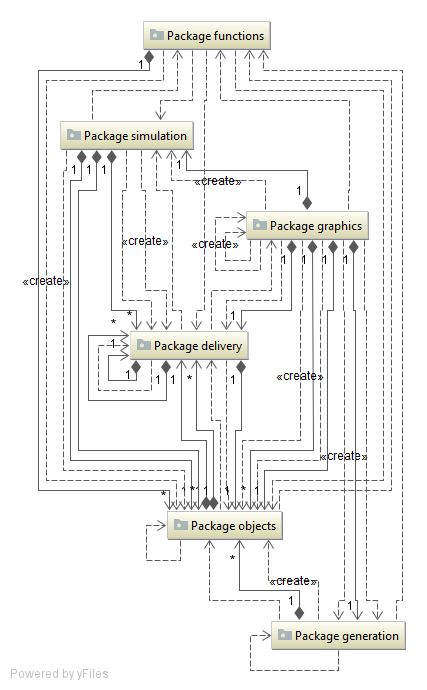
\includegraphics[width=9cm]{uml.png}
\label{fig:uml}
\caption{Zjednodušené UML aplikace (pouze balíčky)}
\end{figure}

\newpage
%
% uživatelská dokumentace
%
\section{Uživatelská dokumentace}
\subsection{Spuštění programu}
Program se spustí jednoduše poklepáním na .jar soubor. Jediná věc, na kterou si uživatel musí dát pozor je, kde program spouští. Program během svého chodu nebo výsledem uživatelské volby vytváří soubory v adresáři, kde se nachází. Program automaticky vytváří soubor typu XML pro statistiky. Mimo tento soubor program může vytvořit 2 textové dokumenty, ukládající data které byly vygenerovány. Tyto soubory jsou vytvořeny pouze pokud uživatel zvolí volbu exportovat data a buď vybere nacházející adresář jako cílový a nebo nevybere žádný adresář a tím pádem se defaultně zvolí adresář, ve kterém je program spuštěn.\newline\newline
\subsection{Ovládání programu}



\begin{figure}[!ht]
\centering
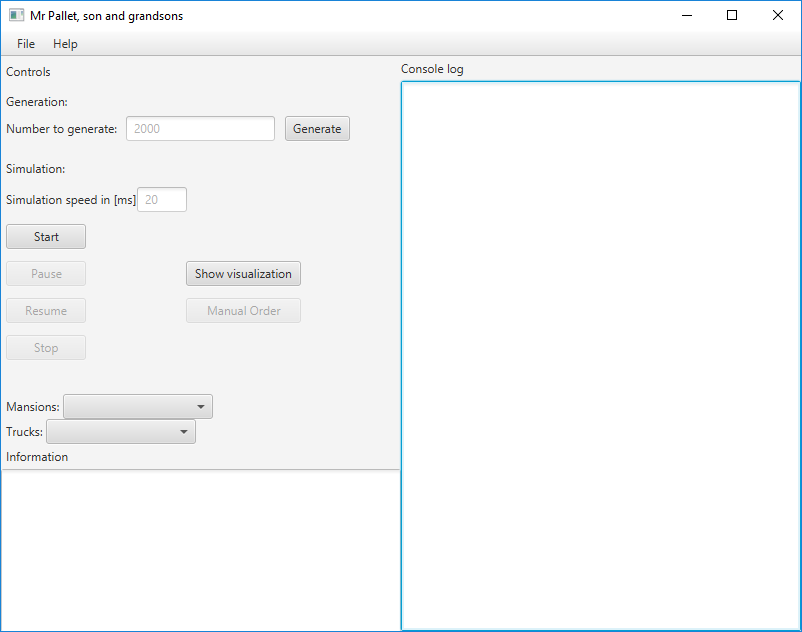
\includegraphics[width=10cm]{guipic.png}
\label{fig:guipic}
\caption{Grafické rozhraní aplikace}
\end{figure}

Po spuštění programu se uživateli otevře uživatelské rozhraní(viz. výše). Některé volby jsou v tuto dobu zablokované a jiné, i přes to že povolené, jsou v tuto dobu nefunkční a budou vracet chybovou hlášku.\newpage
 V tuto chvíli uživatel musí buď importovat data pomocí File-Import * nebo vygenerovat nové data. Pokud uživatel importuje sídla, bude moci pustit simulaci, ale program vytvoří nové hrany a najde nové cesty. Pokud uživatel importuje pouze soubor obsahující matice hran a pokusí se program spustit, tak program reaguje chybovou hláškou, a bude žádat o importování souboru s příslušnými sídly nebo generaci nových dat. Pokud uživatel importuje sdíla i matice, tak po spuštění program vyhledá nejlepší cesty a spustí simulaci. Druhá možnost je generace dat. Pokud uživatel zmáčkne tlačítko generace bez toho, aniž by vyplnit textové pole za popiskem "Number to generate", aplikace začne generovat 2000 sídel a potřebné data pro běh simulace. Uživatel může vybrat počet sídel, který bude použit pro generaci dalších dat a běh simulace, zadáním čísla sídel do již zmíněného textového pole. Pokud uživatel zadá neplatný formát čísla nebo text, program vrací chybovou hlášku.\newline
Pokud program má potřebné data, tak je možné začít simulaci tlačítkem start. Také je možné zobrazit mapu sídel pomocí tlačítka show visualization. Dále má uživatel možnost vybrat si rychlost simulace pomocí textového pole za popiskem "Simulation speed in [ms]", toto pole je samozřejmě ošetřené proti nevhodným formátům a minimální rychlosti simulace. Pokud uživatel nezadá žádnou hodnotu, zvolí se defaultní hodnota. Jakmile je simulace v provozu, je možné zobrazit informace a sídle, které lze vybrat ze seznamu označeným "Mansions". Simulaci jde pozastavit tlačítkem pause. Pokud je simulace pozastavená je možné ji vrátit tlačítkem resume nebo úplně zastavit tlačíkem stop. Pokud je stisknuté tlačítko stop, simulace je kompletně zastavena a pro další spuštění simulace je třeba vygenerovat nebo importvat nové data. Pokud uživatel chce zobrazit informace o určitém trucku, musí simulaci nejdříve pozastavit nebo stopnout, aby se naplnil seznam označený "Trucks". Poslední vlastnot GUI je zobrazení stručného ovládání programu v sekci Help-Instructions.
\newpage
%
% ZÁVĚR
%
\section{Závěr}
Program je dostatečně funkční, aby splnil požadované zadání, ačkoliv stále má znatelné množství chyb. Program by měl být použitelný a relativně snadno upravitelný pro jeho následovné šíření. Ačkoliv si myslím, že program splňuje zadání, tak má hodně nedokonalostí a spoustu funkcí by chtělo ještě vylepšit nebo dodělat.
K volbě algortimů si myslím, že jsme zvolili relativně slušná řešení. Pravděpodobně je možné, že by bylo vhodnější zvolit jiné algortimy v některých případech a během vytváření práce jsem kolikrát přemýšlel, jak by si vedl jiný algoritmus, tak jsem ve výsledku poměrně spokojený s rychlostí programu, ačkoliv je nejspíš možné, že by mohl být ještě znatelně rychlejší.
\end{document}